\newcount\Comments  
\Comments=1   
\documentclass[a4paper,12pt, english]{article}
\usepackage[top=2cm, bottom=2cm, left=2cm, right=2cm]{geometry}

\usepackage{babel}
\usepackage{subfigure}

\usepackage{color}

\definecolor{darkgreen}{rgb}{0,0.5,0}
\definecolor{purple}{rgb}{1,0,1}
\usepackage{graphicx}

\newcommand{\kibitz}[2]{\ifnum\Comments=1\textcolor{#1}{#2}\fi}
% add yourself here:
\newcommand{\ls}[1]{\kibitz{red}      {[Larisa: #1]}}
\newcommand{\cg}[1]  {\kibitz{purple}   {[Crina: #1]}}
\newcommand{\ns}[1]{\kibitz{cyan}     {[Noureddin: #1]}}



\usepackage{listings}
\usepackage{url}
%\usepackage{graphicx}

\usepackage{verbatim}

%\usepackage{caption}
%\usepackage{datetime}

%\onehalfspacing

\begin{document}

\title{Transfer Learning Experiment}
\maketitle

\section{The Idea}
\begin{itemize}
\item \texttt{Target Dataset} is a \textbf{small and labeled} dataset from a certain domain
\item \texttt{Source Dataset(s)} can be one or more \textbf{large and labeled} datasets from \emph{related} domains 
\item If we would like to build a model for the \texttt{Target Dataset} using it alone as \texttt{Training} dataset, then the model will likely perform undesirably as the dataset is quite small!
\item The idea is to make maximum use of the \texttt{Source Datasets} to augment the \texttt{Target Dataset} and classify data from its domain (this is Instance Transfer Learning)
\end{itemize}  

\section{The Data}
\begin{itemize}
\item Two \texttt{Source} datasets TS3-Sapphire.arff and TS6-Sapphire.arff (This is for strain \emph{Plasmodium vivax})
\item The TL algorithm supports having multiple source datasets as it assigns weights to instances as well as source datasets
\item I have done \textbf{two experiments} with two different \texttt{Target} Datasets:
\begin{itemize}
\item Data from the Venus Channel for assay TS6 (This is for strain \emph{Plasmodium falciparum})
\item this dataset has 1435 instances and the number of \texttt{Active} instances is 27
\item details of this experiment are in \textbf{experiment6.pdf}
\item Data from the Sapphire Channel for assay TS7 (This is for strain \emph{Leishmania major}) 
\item this dataset has 1326 instances and the number of \texttt{Active} instances is 12
\item details of this experiment are in \textbf{experiment7.pdf}
\end{itemize}
\item Iteratively, I split each of these two datasets to create \texttt{Target} and \texttt{Test} datasets 
%\item This dataset has 1435 instances and the percentage of \texttt{Active} instances is \textasciitilde2\% (27 instances)
\item I started with a very small \texttt{Target} dataset of all \texttt{Inactives} and doubled the size at each iteration
\item As the size increased, I started to include Active instances (with the same proportion for \emph{Plasmodium falciparum} data)
\item Remember. the \texttt{Target} dataset is used as \texttt{Training} dataset to build TL, NB, J48, SMO and KNN models
\item Details of the various datasets are shown in the following tables:

%\begin{center}
\begin{table}[h]
\centering
    \begin{tabular}{ | l | l | l | }
    \hline
      	\textbf{Exp. No.} & \textbf{Target Dataset (Training)} & \textbf{Test Dataset} \\ \hline
      	1 & Size=3   \begin{scriptsize}(3 Inactive + 0 Active)\end{scriptsize} & Size=1432 \begin{scriptsize}(1405 Inactive + 27 Active)\end{scriptsize}\\ \hline
	2 & Size=6   \begin{scriptsize}(6 Inactive + 0 Active)\end{scriptsize} & Size=1429 \begin{scriptsize}(1402 Inactive + 27 Active)\end{scriptsize}\\ \hline
	3 & Size=12  \begin{scriptsize}(12 Inactive + 0 Active)\end{scriptsize} & Size=1423 \begin{scriptsize}(1396 Inactive + 27 Active)\end{scriptsize}\\ \hline
	4 & Size=24  \begin{scriptsize}(24 Inactive + 0 Active)\end{scriptsize} & Size=1411 \begin{scriptsize}(1384 Inactive + 27 Active)\end{scriptsize}\\ \hline
	5 & Size=49  \begin{scriptsize}(48 Inactive + 1 Active)\end{scriptsize} & Size=1386 \begin{scriptsize}(1360 Inactive + 26 Active)\end{scriptsize}\\ \hline
	6 & Size=98  \begin{scriptsize}(96 Inactive + 2 Active)\end{scriptsize} & Size=1337 \begin{scriptsize}(1312 Inactive + 25 Active)\end{scriptsize}\\ \hline
	7 & Size=196 \begin{scriptsize}(192 Inactive + 4 Active)\end{scriptsize} & Size=1239 \begin{scriptsize}(1216 Inactive + 23 Active)\end{scriptsize}\\ \hline
	8 & Size=392 \begin{scriptsize}(384 Inactive + 8 Active)\end{scriptsize} & Size=1043 \begin{scriptsize}(1024 Inactive + 19 Active)\end{scriptsize}\\ \hline
	9 & Size=784 \begin{scriptsize}(768 Inactive + 16 Active)\end{scriptsize} & Size=651 \begin{scriptsize}(640 Inactive + 11 Active)\end{scriptsize}\\ \hline
    \end{tabular}       
    \caption{Details of Datasets for Strain \emph{Plasmodium falciparum}}
\end{table}
%\end{center}

\begin{table}[h]
\centering
    \begin{tabular}{ | l | l | l | }
    \hline
      	\textbf{Exp. No.} & \textbf{Target Dataset (Training)} & \textbf{Test Dataset} \\ \hline
      	1 & Size=3   \begin{scriptsize}(3 Inactive + 0 Active)\end{scriptsize} & Size=1323 \begin{scriptsize}(1311 Inactive + 12 Active)\end{scriptsize}\\ \hline
	2 & Size=6   \begin{scriptsize}(6 Inactive + 0 Active)\end{scriptsize} & Size=1320 \begin{scriptsize}(1308 Inactive + 12 Active)\end{scriptsize}\\ \hline
	3 & Size=12  \begin{scriptsize}(12 Inactive + 0 Active)\end{scriptsize} & Size=1314 \begin{scriptsize}(1302 Inactive + 12 Active)\end{scriptsize}\\ \hline
	4 & Size=25  \begin{scriptsize}(24 Inactive + 1 Active)\end{scriptsize} & Size=1301 \begin{scriptsize}(1290 Inactive + 11 Active)\end{scriptsize}\\ \hline
	5 & Size=50  \begin{scriptsize}(48 Inactive + 2 Active)\end{scriptsize} & Size=1276 \begin{scriptsize}(1266 Inactive + 10 Active)\end{scriptsize}\\ \hline
	6 & Size=100 \begin{scriptsize}(96 Inactive + 4 Active)\end{scriptsize} & Size=1226 \begin{scriptsize}(1218 Inactive + 8 Active)\end{scriptsize}\\ \hline
	7 & Size=200 \begin{scriptsize}(192 Inactive + 8 Active)\end{scriptsize} & Size=1239 \begin{scriptsize}(1122 Inactive + 4 Active)\end{scriptsize}\\ \hline	
    \end{tabular}  
    \caption{Details of Datasets for Strain \emph{Leishmania major}}     
\end{table}

\end{itemize}  

\newpage
\subsection{Algorithm Names in Results Tables:}
I have abbreviated column names in the tables to save display space:\\
TL = Transfer Learning,\\
NB = Naive Bayes,\\
J48 = The J48 Decision Trees,\\
SMO = Support Vector Machine,\\
IBk = Instance Based (k-Nearest Neighbour)


\subsection{Column Names in Results Tables:}
I have abbreviated column names in the tables to save display space. In order from left to right, they're as follows:\\
corr = Percentage of Correct guesses,\\
inco = Percentage of Incorrect guesses,\\
auc = Area Under the Curve (for class Active),\\
k = Kappa statistic,\\
mae = Mean Abs Error,\\
rmse = Root Mean Squared Error,\\
rae = Relative Abs Error,\\
rrse = Root Relative Squared Error,\\
prec = Precision (for class Active),\\
rec = Recall (for class Active),\\
fM = F-Measure (for class Active),\\
eR = Error Rate\\
%\newpage



%\date{Mar 2014}
%\author{By: Noureddin Sadawi}
%\maketitle

%\large
\begin{comment}
\section{Scenario}
Let us assume that we have a \textbf{small} labeled dataset from one domain (we are going to call this dataset the $Target Dataset$) and [usually] it is costly to obtain new labelled data from the same domain (so the quantity is limited). \\

Also, let us also assume that we have one or more \textbf{large} and labeled datasets from a \textbf{\emph{related}} domains (we are going to call these datasets the $Source Datasets$) and [usually] it is affordable to obtain new labelled data from these domains.\\

%In classification learning, it is usually assumed that training and test sets have identical distributions!\\

If we would like to build a model for the $Target Dataset$ using it alone, then the model will likely perform undesirably as the dataset is quite small!\\

The idea is to make maximum use of the $Source Datasets$  to build a model for the $Target Dataset$ and classify data from its domain. In other words, we want to reuse data from the source tasks to augment the target task's training data (this is Instance Transfer Learning)\\

In this experiment, I have used the technique explained in a paper called \textit{"Selective Transfer Between Learning Tasks Using Task-Based Boosting"} to gain knowledge from the $Source$ data and use it in training a classifier for the $Target$ data. The proposed algorithm is called $TransferBoost$ and it is based on the classical $AdaBoost$ Algorithm!\\

\section{How TransferBoost Works (from the abovementioned paper)}
As the source and target data are from different but related domains, the two tasks (i.e. source and target) have different distributions. Yet, some of the source tasks' data could have been drawn from the target task's distribution. Such data could then be used as additional training data for the target task.\\

$TransferBoost$ attempts to automatically select individual data from the source tasks to augment the target task’s training data. It automatically determines the weight to assign to each source instance in learning the target task's model, building on the $AdaBoost$ algorithm. TransferBoost iteratively constructs an ensemble of classifiers, reweighting both the source and target data via two types of boosting: individual and task-based.\\
It increases the weight of individual mispredicted instances following AdaBoost. In parallel, it also performs task-based boosting by reweighting all instances from each source task based on their aggregate transfer to the target task.\\

In effect, TransferBoost increases the weight of source tasks that show positive transfer to the target task, and then reweights the instances within each task via AdaBoost. 




\section{Experiment I}
\subsection{The Data}
\begin{itemize}
\item By looking at the table provided with the Eve data, I have extracted and merged labeled data from the Sapphire Channel (Sapphire Active/Inactive) for assays TS3 and TS6. This is for strain \emph{Plasmodium vivax}. This is going to be our $Source Dataset$

\item I have also extracted labeled data from the Venus Channel (Venus Active/Inactive) for assay TS6. This is for strain \emph{Plasmodium falciparum}. This is going to be our $Target Dataset$
\item I have split the $Target Dataset$ into two subdatasets. One for training and one for testing. Notice that this training subdataset is going to be our actual $Target Dataset$
\item Now our datasets look like:
   \begin{itemize}
	\item $Source Dataset$ has 2781 instances (for Pv from TS3 and TS6 -- file TS3-TS6-Pv-Source.arff -- 2737 Inactive + 44 Active)
	\item $Target Dataset$ has 46 instances (for Pf from TS6 -- file TS6-Pf-Target.arff -- 41 Inactive + 5 Active)
	\item $Test Dataset$ has 1389 instances (for Pf from TS6 -- file TS6-Test-Pf.arff -- 1367 Inactive + 22 Active)
	\item $Target Dataset2$ has 301 instances (for Pf from TS6 -- file TS6-Pf-Target2.arff -- 289 Inactive + 11 Active). I have randomly chosen instances of this dataset from the $Test Dataset$ WITHOUT removing them from the $Test Dataset$!
   \end{itemize}  
\end{itemize}  

\subsection{Experimental Setup}
The authors of the paper have provided the java source code of their implementation so I have downloaded it, plugged it into WEKA's source code and recompiled WEKA.\\
Remember that our $Target Dataset$ is quite small and our $Source Dataset$ is large and from a related domain.\\
We will use our $Test Dataset$ for evaluation (it is from the same domain as $Target Dataset$)\\

Here is what I have done:
\begin{itemize}
\item I have built a classification model with the TransferBoost Algorithm using both the $Target$ and $Source$ Datasets to carry out Transfer Learning. I used \emph{Decision Stump} as the base classifier.
\item I have built classification models with WEKA's NaiveBayes, SVM, KNN and J48 Decision Trees using the $Target Dataset$ only. This is because usually we build models using data from the same domain!
\end{itemize}

\subsection{Column Names:}
I have abbreviated column names in the following tables to save display space. In order from left to right, they're as follows:\\
Percentage of Correct guesses,\\
Percentage of Incorrect guesses,\\
Area Under the Curve (for class Active),\\
Kappa statistic,\\
Mean Abs Error,\\
Root Mean Squared Error,\\
Relative Abs Error,\\
Root Relative Squared Error,\\
Precision (for class Active),\\
Recall (for class Active),\\
F-Measure (for class Active),\\
Error Rate\\


\subsection{Experimental Stat Results 1}
In this experiment I did 10 fold cross validation using the target dataset (remember the TL classifier needs the target dataset and at least one source dataset)
\begin{small}
\begin{center}
    \begin{tabular}{ | l | l | l | l | l | l | l | l | l | l | l | l | l |}
    \hline
      	& corr & incorr  & auc & kap & mae & rmse & rae & rrse & prec & rec & fm & err rate\\ \hline
      	TL & 95.65\% & 4.34\% & 0.97 & 0.72 & 0.04 & 0.21 & 23.81\% & 67.52\% & 1 & 0.6 & 0.74 & 0.04\\ \hline
	NB & \textbf{97.82}\% & 2.17\% & \textbf{1} & 0.89 & 0.02 & 0.14 & 10.39\% & 46.77\% & 0.83 & 1 & 0.9 & 0.02\\ \hline
	J48 & 91.3\% & 8.69\% & 0.86 & 0.61 & 0.08 & 0.29 & 41.56\% & 93.55\% & 0.57 & 0.8 & 0.66 & 0.08\\ \hline
	SMO & 93.47\% & 6.52\% & 0.7 & 0.54 & 0.06 & 0.25 & 31.17\% & 81.02\% & 1 & 0.4 & 0.57 & 0.06\\ \hline
	IBk & 91.3\% & 8.69\% & \textbf{1} & 0.3 & 0.07 & 0.21 & 35.22\% & 67.32\% & 1 & 0.2 & 0.33 & 0.08\\ \hline  
    \end{tabular}       
\end{center}
\end{small}


\subsection{Experimental Stat Results 2}
In this experiment I did 10 fold cross validation using the other target dataset ( $Target Dataset2$ which has 289 Inactive + 12 Active)
\begin{small}
\begin{center}
    \begin{tabular}{ | l | l | l | l | l | l | l | l | l | l | l | l | l |}
    \hline
      	& corr & incorr  & auc & kap & mae & rmse & rae & rrse & prec & rec & fm & err rate\\ \hline
	TL & 98\% & 1.99\% & \textbf{0.99} & 0.75 & 0.01 & 0.12 & 22.81\% & 62.47\% & 0.71 & 0.83 & 0.76 & 0.01\\ \hline
	NB & 96.34\% & 3.65\% & \textbf{0.99} & 0.66 & 0.03 & 0.19 & 45.76\% & 97.42\% & 0.52 & 1 & 0.68 & 0.03\\ \hline
	J48 & 98\% & 1.99\% & 0.69 & 0.71 & 0.02 & 0.14 & 31.9\% & 72.82\% & 0.8 & 0.66 & 0.72 & 0.01\\ \hline
	SMO & \textbf{98.67}\% & 1.32\% & 0.83 & 0.79 & 0.01 & 0.11 & 16.67\% & 58.88\% & 1 & 0.66 & 0.8 & 0.01\\ \hline
	IBk & 98\% & 1.99\% & 0.9 & 0.65 & 0.02 & 0.12 & 26.73\% & 62\% & 1 & 0.5 & 0.66 & 0.01\\ \hline
    \end{tabular}       
\end{center}
\end{small}

\subsection{Experimental Stat Results 3}
In this experiment I did 10 fold cross validation using the test dataset
\begin{small}
\begin{center}
    \begin{tabular}{ | l | l | l | l | l | l | l | l | l | l | l | l | l |}
    \hline
& corr & incorr  & auc & kap & mae & rmse & rae & rrse & prec & rec & fm & err rate\\ \hline    
TL & 99.56\% & 0.43\% & \textbf{0.99} & 0.86 & 0 & 0.05 & 12.53\% & 42.36\% & 0.86 & 0.86 & 0.86 & 0\\ \hline
NB & 97.55\% & 2.44\% & \textbf{0.99} & 0.55 & 0.02 & 0.15 & 76.65\% & 125.25 & 0.39 & 1 & 0.56 & 0.02\\ \hline
J48 & 99.49\% & 0.5\% & 0.89 & 0.83 & 0 & 0.06 & 19.11\% & 55.34\% & 0.85 & 0.81 & 0.83 & 0\\ \hline
SMO & \textbf{99.64}\% & 0.35\% & 0.9 & 0.87 & 0 & 0.05 & 11.27\% & 48.05\% & 0.94 & 0.81 & 0.87 & 0\\ \hline
IBk & 99.42\% & 0.57\% & 0.97 & 0.78 & 0 & 0.06 & 18.53\% & 49.37\% & 0.93 & 0.68 & 0.78 & 0\\ \hline      
    
    \end{tabular}       
\end{center}
\end{small}

\subsection{Experimental Stat Results 4}
In this experiment I did evaluation using the test dataset (built models using the $Target Dataset$ and used the test dataset for the validation)
\begin{small}
\begin{center}
    \begin{tabular}{ | l | l | l | l | l | l | l | l | l | l | l | l | l |}
    \hline
	& corr & incorr  & auc & kap & mae & rmse & rae & rrse & prec & rec & fm & err rate\\ \hline    
	TL & \textbf{99.56}\% & 0.43\% & \textbf{0.99} & 0.87 & 0 & 0.06 & 3.35\% & 38.34\% & 0.8 & 0.95 & 0.87 & 0\\ \hline  
	NB & 91.72\% & 8.27\% & 0.95 & 0.25 & 0.08 & 0.28 & 60.47\% & 173.46\% & 0.16 & 1 & 0.27 & 0.08\\ \hline  
	J48 & 98.2\% & 1.79\% & \textbf{0.99} & 0.62 & 0.01 & 0.13 & 13.14\% & 80.89\% & 0.46 & 1 & 0.63 & 0.01\\ \hline  
	SMO & 99.28\% & 0.71\% & 0.97 & 0.8 & 0 & 0.08 & 5.25\% & 51.16\% & 0.7 & 0.95 & 0.8 & 0\\ \hline  
	IBk & 99.35\% & 0.64\% & 0.95 & 0.73 & 0.01 & 0.07 & 9.61\% & 44.37\% & 1 & 0.59 & 0.74 & 0 \\ \hline   		    
    \end{tabular}       
\end{center}
\end{small}

\subsection{Experimental Stat Results 5}
In this experiment I did evaluation using the test dataset (built models using the $Target Dataset2$ (which is larger that Target Dataset) and used the test dataset for the validation)
\begin{small}
\begin{center}
    \begin{tabular}{ | l | l | l | l | l | l | l | l | l | l | l | l | l |}
    \hline
	& corr & incorr  & auc & kap & mae & rmse & rae & rrse & prec & rec & fm & err rate\\ \hline    
	TL & \textbf{99.85}\% & 0.14\% & \textbf{0.99} & 0.95 & 0 & 0.03 & 8.95\% & 27.97\% & 0.95 & 0.95 & 0.95 & 0\\ \hline  
	NB & 98.99\% & 1\% & \textbf{0.99} & 0.75 & 0 & 0.09 & 31.12\% & 79.16\% & 0.61 & 1 & 0.75 & 0.01\\ \hline  
	J48 & 99.42\% & 0.57\% & 0.79 & 0.8 & 0.01 & 0.07 & 31.49\% & 59.43\% & 0.85 & 0.77 & 0.8 & 0\\ \hline  
	SMO & 99.64\% & 0.35\% & 0.88 & 0.86 & 0 & 0.05 & 11.3\% & 48.05\% & 1 & 0.77 & 0.87 & 0\\ \hline  
	IBk & 99.49\% & 0.5\% & \textbf{0.99} & 0.8 & 0 & 0.05 & 19.23\% & 44.66\% & 1 & 0.68 & 0.81 & 0 \\ \hline  		    
    \end{tabular}       
\end{center}
\end{small}


\subsection{Experimental Results}
After building the models as explained above, I have evaluated them using the $Test Dataset$ which is of the same domain as the $Target Dataset$. I have counted Actual vs Predicted results.\\
The following table shows how many miss-classifications each model makes:\\ 
\begin{center}
    \begin{tabular}{ | l | l | l | p{5cm} | l |}
    \hline
    TransferBoost & NaiveBayes & SVM & KNN & J48 Decision Trees \\ \hline
    6 & 115 & 10 & 9 & 25\\
    \hline
    \end{tabular}       
\end{center}

Observe that the TransferBoost model (the one that does Transfer Learning) makes less classification errors meaning it outperforms models built using the $Target Dataset$ alone.

\newpage


\section{Experiment II}
In this experiment, I am going to try and do TL at assay level. Meaning I will use Active/Inactive labelled datasets from the eve data (assays TS3,4,5,6,7)
\subsection{The Data}
\begin{itemize}
\item For the $Source Dataset$, I have used TS3 (1346 instances (4 Active) -- file TS3-Labeled.arff)
\item I have randomly split TS5 into two datasets:
\begin{itemize}
\item $Target Dataset$ ... 278 instances (3 Active + 275 Inactive) -- file TS5-Labeled-Target.arff
\item $Test Dataset$ ... 1116 instances (5 Active) -- file TS5-Labeled-Test.arff
\end{itemize}
\end{itemize}  

\subsection{Experimental Setup}
Exactly the same as Experiment I

\subsection{Experimental Stat Results 1}
In this experiment I did 10 fold cross validation using the target dataset (remember the TL classifier needs the target dataset and at least one source dataset)
\begin{small}
\begin{center}
    \begin{tabular}{ | l | l | l | l | l | l | l | l | l | l | l | l | l |}
    \hline
      & corr & incorr  & auc & kap & mae & rmse & rae & rrse & prec & rec & fm & err rate\\ \hline
      TL  & \textbf{99.64}\% & 0.35\% & 0.68 & 0.79 & 0 & 0.05 & 14.34\% & 57.83\% & 1 & 0.66 & 0.8 & 0\\ \hline
      NB  & 98.2\%  & 1.79\% & 0.67 & 0.43 & 0.01 & 0.13 & 76.73\% & 130.29\% & 0.33 & 0.66 & 0.44 & 0.01\\ \hline
      J48 & 98.56\% & 1.43\% & 0.66 & 0.32 & 0.01 & 0.12 & 61.86\% & 117.27\% & 0.33 & 0.33 & 0.33 & 0.01\\ \hline
      SMO & 98.56\% & 1.43\% & 0.66 & 0.32 & 0.01 & 0.11 & 57.1\% & 115.67\% & 0.33 & 0.33 & 0.33 & 0.01\\ \hline
      IBk & 98.92\% & 1.07\% & \textbf{0.86} & 0 & 0.01 & 0.09 & 48.77\% & 89.55\% & 0 & 0 & 0 & 0.01\\ \hline

    
    
    \end{tabular}       
\end{center}
\end{small}

\subsection{Experimental Stat Results 2}
In this experiment I did 10 fold cross validation using the test dataset
\begin{small}
\begin{center}
    \begin{tabular}{ | l | l | l | l | l | l | l | l | l | l | l | l | l |}
    \hline
& corr & incorr  & auc & kap & mae & rmse & rae & rrse & prec & rec & fm & err rate\\ \hline    
TL & 99.73\% & 0.26\% & 0.99 & 0.66 & 0 & 0.04 & 26.09\% & 74.67\% & 0.75 & 0.6 & 0.66 & 0\\ \hline
NB & 98.65\% & 1.34\% & 0.99 & 0.39 & 0.01 & 0.11 & 135.78\% & 173.48\% & 0.25 & 1 & 0.4 & 0.01\\ \hline
J48 & \textbf{99.82}\% & 0.17\% & 0.89 & 0.79 & 0 & 0.04 & 18.1\% & 63.34\% & 0.8 & 0.8 & 0.8 & 0\\ \hline
SMO & 99.73\% & 0.26\% & 0.79 & 0.66 & 0 & 0.05 & 27.15\% & 77.58\% & 0.75 & 0.6 & 0.66 & 0\\ \hline
IBk & 99.55\% & 0.44\% & \textbf{1} & 0 & 0 & 0.04 & 32.77\% & 61.41\% & 0 & 0 & 0 & 0\\ \hline
    
    \end{tabular}       
\end{center}
\end{small}

\subsection{Experimental Stat Results 3}
In this experiment I did evaluation using the test dataset (built models using the target dataset and used the test dataset for the validation)
\begin{small}
\begin{center}
    \begin{tabular}{ | l | l | l | l | l | l | l | l | l | l | l | l | l |}
    \hline
& corr & incorr  & auc & kap & mae & rmse & rae & rrse & prec & rec & fm & err rate\\ \hline    
TL & \textbf{99.73}\% & 0.26\% & \textbf{0.99} & 0.57 & 0 & 0.05 & 14.43\% & 76.81\% & 1 & 0.4 & 0.57 & 0\\ \hline  
NB & 99.28\% & 0.71\% & 0.79 & 0.49 & 0 & 0.08 & 38.46\% & 125.43\% & 0.36 & 0.8 & 0.5 & 0\\ \hline
J48 & 99.55\% & 0.44\% & 0.69 & 0.44 & 0 & 0.06 & 24.03\% & 91.42\% & 0.5 & 0.4 & 0.44 & 0\\ \hline
SMO & \textbf{99.73}\% & 0.26\% & 0.7 & 0.57 & 0 & 0.05 & 14.42\% & 76.81\% & 1 & 0.4 & 0.57 & 0\\ \hline
IBk & 99.55\% & 0.44\% & \textbf{0.99} & 0 & 0 & 0.04 & 23.05\% & 73.11\% & 0 & 0 & 0 & 0  \\ \hline
    
    \end{tabular}       
\end{center}
\end{small}

\subsection{Experimental Results}
After building the models as explained above, I have evaluated them using the $Test Dataset$ which is of the same domain as the $Target Dataset$. I have counted Actual vs Predicted results.\\
The following table shows how many miss-classifications each model makes:\\ 
\begin{center}
    \begin{tabular}{ | l | l | l | p{5cm} | l |}
    \hline
    TransferBoost & NaiveBayes & SVM & KNN & J48 Decision Trees \\ \hline
    3 & 8 & 3 & 5 & 5\\
    \hline
    \end{tabular}       
\end{center}

Observe that the TransferBoost model (the one that does Transfer Learning) makes less classification errors meaning it outperforms models built using the $Target Dataset$ alone.

\begin{figure}[htp]
  \begin{center}
    \subfigure[TransferBoost TL]{\label{fig:a2}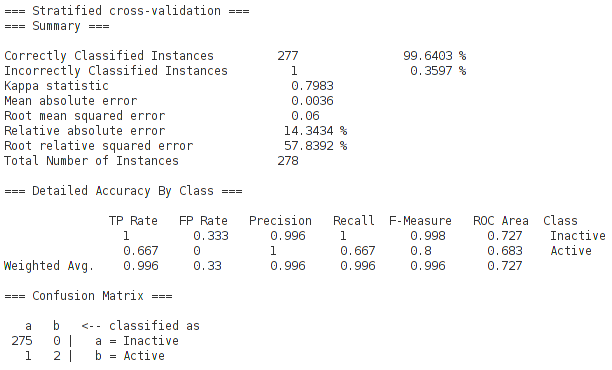
\includegraphics[scale=0.4]{figs/exp2-10CV}}\\
    \subfigure[NaiveBayes]{\label{fig:b2}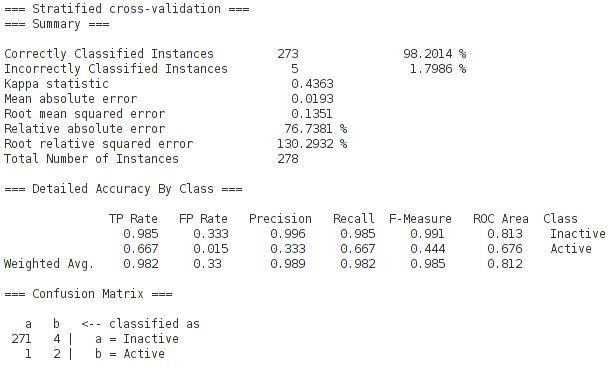
\includegraphics[scale=0.4]{figs/exp2-NB-10CV}} \\
    \subfigure[SVM]{\label{fig:c2}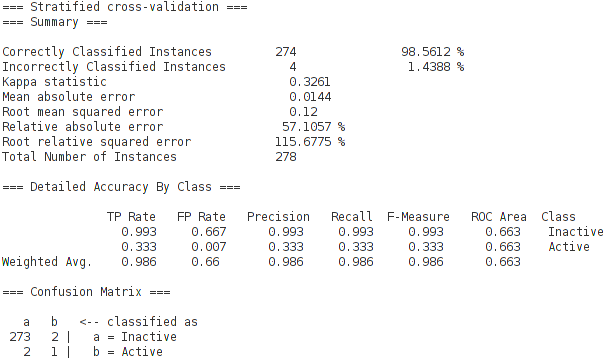
\includegraphics[scale=0.4]{figs/exp2-SVM-10CV}}\\
    \subfigure[J48 Decision Tree]{\label{fig:d2}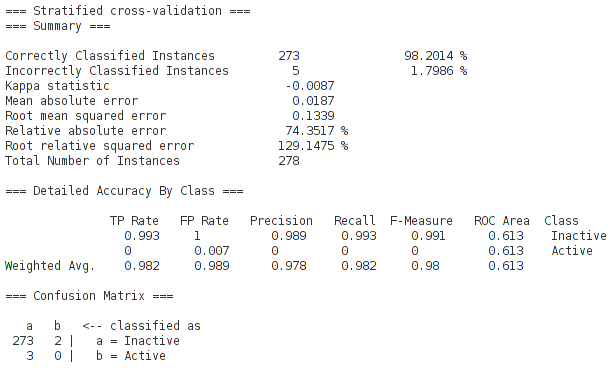
\includegraphics[scale=0.4]{figs/exp2-J48-10CV}}
  \end{center}
  \caption{Stats after running 10 Fold CV}
  \label{fig:stats2}
\end{figure}
\end{comment}
		
\end{document}
